\documentclass{beamer}
\usepackage{graphicx}

\newcommand*{\rom}[1]{\expandafter\@slowromancap\romannumeral #1@}
\newcommand{\ts}{\textsuperscript}


\usetheme{Boadilla}

% items enclosed in square brackets are optional; explanation below
\title[Privacy in Art, Books, and Film]{I've Got Nothing to Hide: \\
  Exploring Privacy in Art, Books, and Film}
\author[Josh Datko]{Joshua Datko}
\institute[Drexel]{
  Department of Computer Science\\
  Drexel University\\
  Philadelphia, PA 19103\\[1ex]
  \texttt{jbd65@drexel.edu}
}
\date[September 2013]{September 28, 2013}

\setbeamertemplate{bibliography item}[text]




\begin{document}

%--- the titlepage frame -------------------------%
\begin{frame}[plain]
  \titlepage
\end{frame}


\begin{frame}
  \frametitle{Motivation}

  \begin{itemize}
  \item Tor runs on volunteers.
  \item Tor needs more volunteers.
  \item Tor should incentivize relay and bridge operators.
  \end{itemize}

  \begin{block}{People like money.}
    Provide incentives for Tor server operators through Bitcoin.
  \end{block}
\end{frame}

\begin{frame}

\frametitle{\emph{The Neighbors} by Arne Svenson}

\begin{itemize}
\item Photographer takes pictures of his neighbors, without their
  knowledge,  in Tribeca (NYC).
\item Two neighbors sued.  Their children were in the photos.
\item Court ruled the artist was protected under the First Amendment.


\end{itemize}

\begin{block}{I have nothing to hide.}
    Unless you take a picture of me and call it art!
  \end{block}

\end{frame}

\begin{frame}
\frametitle{\emph{Neighbors}}


    \begin{columns}[c] % the "c" option specifies center vertical alignment
    \column{.5\textwidth} % column designated by a command
    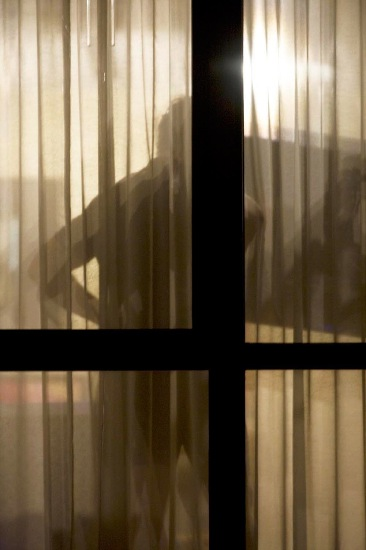
\includegraphics[width=\textwidth,height=0.8\textheight,keepaspectratio]{img/10_website_IMG_4763}

    \column{.5\textwidth}
    \begin{figure}
    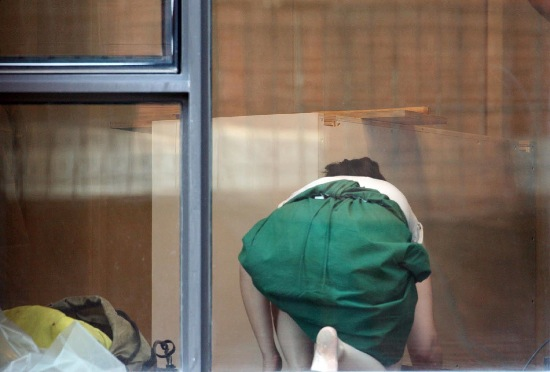
\includegraphics[width=\textwidth,height=0.8\textheight,keepaspectratio]{img/4_website_IMG_3013.jpg}
    \caption{Photos Copyright Arne Svenson}
    \end{figure}

    \end{columns}


\end{frame}

\begin{frame}

\frametitle{\emph{Bleeding Edge} by Thomas Pynchon}

\begin{itemize}
\item Released last week
\item Very Pynchon.  Avant-garde literature ala \emph{Gravity's
  Rainbow}
\item Set in early 2001 in NYC.  In the post tech bust but before
  9/11.
\item Explores the idea of getting ``lost'' on the Internet and how
  that ended with 9/11.
\end{itemize}
\end{frame}



% \begin{frame}
% \frametitle{Survival Curve}
%   \includegraphics[width=\textwidth,height=0.8\textheight,keepaspectratio]{survival}
% \end{frame}
%% \begin{frame}
%%   \frametitle{Bitcoin}

%%   Bitcoin is a peer-to-peer electronic currency based on
%%   proof-of-work. \cite{nakamoto2009bitcoin}

%%   \includegraphics[width=\textwidth,height=0.8\textheight,keepaspectratio]{bitcoin_volume}

%% \end{frame}

%% \begin{frame}
%%   \frametitle{Can Bitcoin provide incentives?}

%%   Bitcoin is not
%%   anonymous.\cite{journals/iacr/AndroulakiKRSC12} \cite{journals/corr/abs-1107-4524}

%%   Combining Bitcoin as is with Tor would expose Tor users.  We seek to
%%   investigate alternative means of payments.
%%   \begin{itemize}
%%   \item Tor client joins a Bitcoin mining pool and payment goes
%%     directly to the Tor Server?
%%   \item Can we use Zerocoin? \cite{Miers:2013:ZAD:2497621.2498124}
%%     \end{itemize}

%%   \begin{block}{Anonymity}
%%     Tor incentives can't compromise anonymity!!
%%   \end{block}
%% \end{frame}

%% \begin{frame}
%%   \frametitle{Approach}


%%   \begin{itemize}
%%   \item Compare BitTor to other incentive
%%     systems.\cite{Jansen:2010:RNT:1866307.1866344}\cite{lira-ndss13}\cite{raykova-pet2008}
%%   \item Investigate Bitcoin payment methods.
%%   \item Provide anonymity analysis.
%%     \item Prototype BitTor and investigate performance

%%     \end{itemize}

%%   \begin{block}{Live and dynamic systems}
%%     Bitcoin = money, Tor = privacy $\rightarrow$ testing to be done ``offline.''
%%   \end{block}
%% \end{frame}



%% \begin{frame}[allowframebreaks]

%%   \frametitle{References}
%%   \begin{small}
%%   \phantomsection
%%   \addcontentsline{toc}{section}{\bibname}
%%   \bibliographystyle{acm}
%%   \bibliography{bitcoin,tor}
%%   \end{small}

%% \end{frame}



\end{document}

%%% Local Variables:
%%% mode: latex
%%% TeX-master: t
%%% End:
